\documentclass[14pt]{extarticle}
\usepackage{amsmath}
\usepackage{amssymb}
%\usepackage{tikz}
%\usetikzlibrary{calc}
%\usetikzlibrary{trees}
\usepackage{hyperref}
\usepackage{graphicx}
\graphicspath{ {../../chap09/} }
\usepackage[top=0.75in, bottom=0.75in, left=0.75in, right=0.75in]{geometry}
\newcommand*{\Scale}[2][4]{\scalebox{#1}{\ensuremath{#2}}}%
\usepackage[shortlabels]{enumitem}
\usepackage[most]{tcolorbox}
\definecolor{bg}{RGB}{255,249,227}
% \usepackage{showframe}
\title{\vspace{-5ex}Math 208 Section 9.1}
\date{\vspace{-10ex}}
%\usepackage{multicol}
%\setlength{\columnsep}{1cm}
\setlength{\parindent}{0pt}
%\usepackage{wrapfig}
\usepackage{parskip}
\setlength{\parskip}{10pt} % 1ex plus 0.5ex minus 0.2ex}
%\usepackage{ragged2e}


\begin{document}
	\maketitle		
	\section*{Homework, Reading, and Other}
	\begin{itemize}
		\item Section 9.1
		\item Section 9.2
	\end{itemize}

	\section{Goals}
	\begin{itemize}
		\item What is a limit?
		\item Analyze and evaluate limits
		\item Identify indeterminate form limits
	\end{itemize}
		
\section{Section 9.1: Limits}
\subsection{Introduction}
Chapter 9 starts our peek into the large topic of Calculus. Algebra considers the world as a static object. Calculus considers mathematical models as dynamic.

Calculus is used in the physical sciences, in business, economics, life sciences, and social sciences -- any discipline that seeks to understand dynamic phenomena.

Chapter 9 introduces the derivative, one of the two key concepts in calculus. The other key concept is the integral. Each of these concepts depend on the notion of a \textit{limit}.

\subsection{Review: Functions and Graphs}
The graph of a function is the graph of the set of all ordered pairs that satisfy the function.

\textbf{Example $\mathbf{f(x) =2x–1}$:} The graph of this function is the set of all ordered pairs $(x, f(x))$.
	\begin{center}
		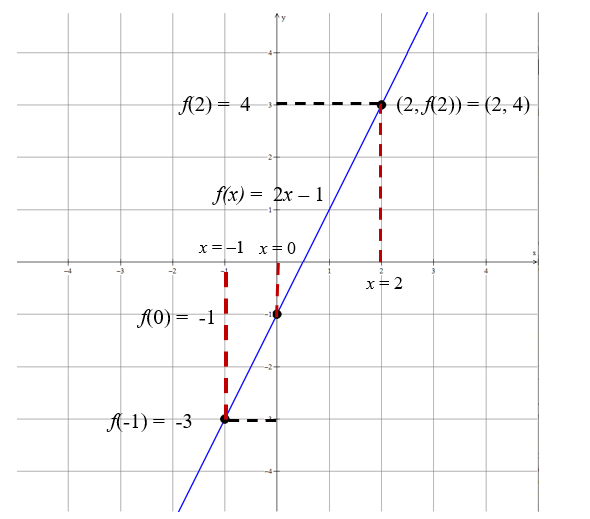
\includegraphics[width=0.7\textwidth]{9-1-intro-1}
	\end{center}
When $x=2, f(2) = 3$ and then $(x, f(x)) = (2, f(2)) = (2, 3)$ is a point on the graph of f.

For $x = 0,  f(0) = –1$ and $(0, f(0)) = (0, –1)$ is on the graph of f.

For $x = –1,  f(–1) = –3$ and $(–1, f(–1)) = (–1, –3)$ is on the graph of f.

Consider what happens when we select values for $x$, closer and closer to $2$.
\begin{center}

\begin{tabular}{|r|c|c|c|c|c|c|c|c|c|}
	\hline
	$\mathbf{x}$ & 1.5 & 1.9 & 1.99 & 1.999 & 2 & 2.001 & 2.01 & 2.1 & 2.5 \\
	\hline
	$\mathbf{f(x)}$ & 2 & 2.8 & 2.98 & 2.998 & \hspace{2cm} & 3.002 & 3.02 & 3.2 & 4 \\
	\hline
\end{tabular}
\end{center}
The value of the function seems to approach $3$. This is the limit concept. In symbols, this is
$$\lim_{x\to 2} f(x)=3$$

\subsection{Limits}
You have now seen an example of a limit, let's consider this further.
\\\\
\textbf{Example $\mathbf{f(x) =x+2}$:} The graph of this function is the set of all ordered pairs $(x, f(x))$. How does this function behave as x gets close to 2?
\begin{center}
	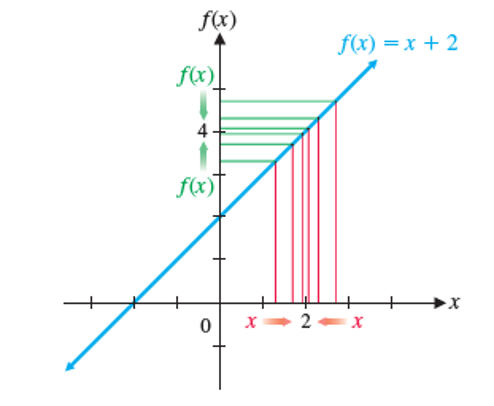
\includegraphics[width=0.5\textwidth]{9-1-intro-2}
\end{center}
From the graph, we may determine that as $x\to 2$ we have that $f(x)\to 4$. Mathematically, this is, \textit{the limit of $f(x)$ as $x$ approaches 2 is 4}, or $$\lim_{x\to 2} f(x) = 4$$
\begin{center}
	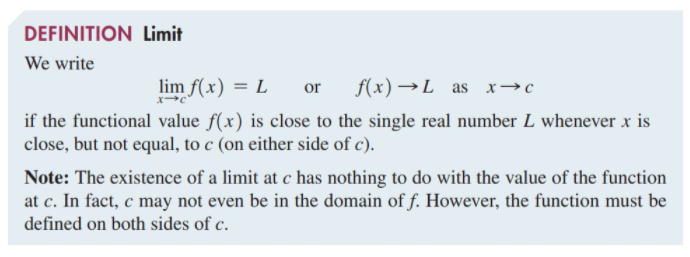
\includegraphics[width=0.9\linewidth]{9-1-1}
\end{center}
This is usually what we mean by limit of a function but we also have a more specialized term and that is one-sided limits. Instead of $x \to c$, we have $x \to c^-$ and $x\to c^+$. These mean as $x$ gets closer to $c$ from the left ($c^-$) and from the right ($c^+$) respectively.



\cleardoublepage
\begin{center}
	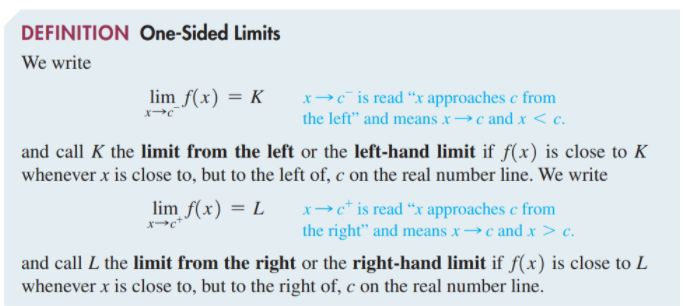
\includegraphics[width=0.9\linewidth]{9-1-2a}
\end{center}
Why do we need one-sided limits? Consider the following. Recall the absolute value function,
\begin{align*}
	f(x) = \vert x \vert = \begin{cases}
		-x  & \text{for } x < 0 \\
		x & \text{for } x \geq 0
	\end{cases}
\end{align*}
Let $h(x)=\frac{\vert x \vert}{x}$. Explore the limit as $x\to 0^-$ and $x\to 0^+$.
\begin{center}
	\begin{tabular}{|r|c|c|c|c|c|c|c|c|c|}
		\hline
		$\mathbf{x}$ & -1 & -0.1 & -0.01 & -0.001 & 0 & 0.001 & 0.01 & 0.1 & 1 \\
		\hline
		$\mathbf{h(x)}$ & -1 & -1 & -1 & -1 & \hspace{2cm} & 1 & 1 & 1 & 1 \\
		\hline
	\end{tabular}
\end{center}
\begin{center}
	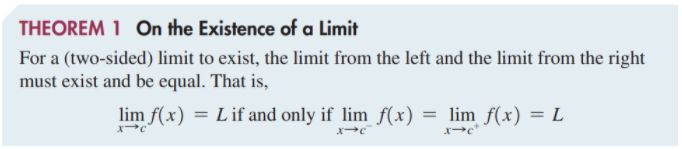
\includegraphics[width=0.9\linewidth]{9-1-2b}
\end{center}
Using this Theorem, we state that since:
$$ \lim_{x\to 0^-} h(x) \neq \lim_{x\to 0^+} h(x)  $$
the $$\lim_{x\to 0}h(x)= \text{ Does Not Exist}$$

\begin{center}
	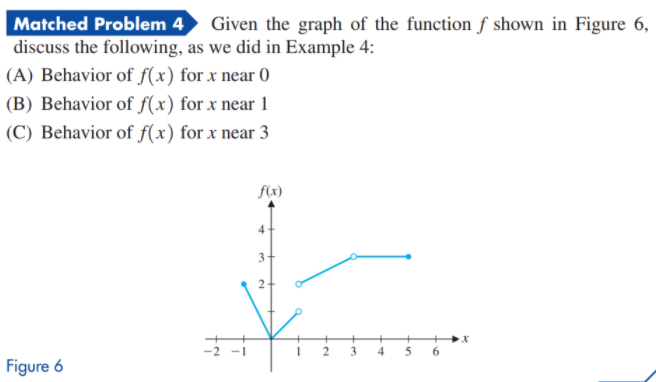
\includegraphics[width=0.9\linewidth]{9-1-3}
\end{center}

\subsection{Properties of Limits}
\begin{center}
	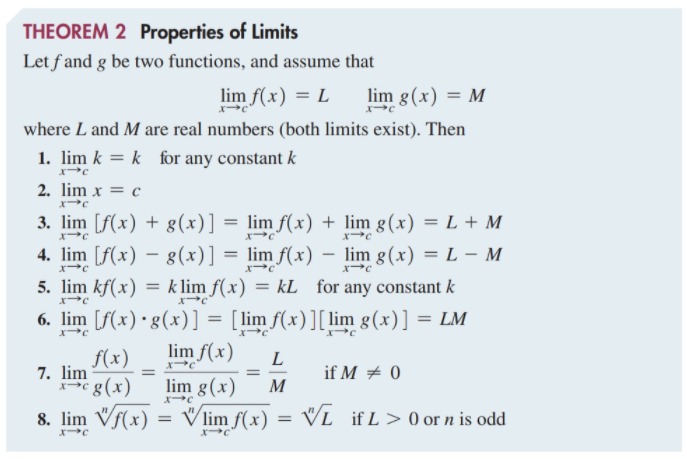
\includegraphics[width=0.9\linewidth]{9-1-4}
\end{center}
Look these over and be sure to use these when doing the examples and your homework.
\subsubsection{Examples} Find the limit, if it exists.
\begin{align*}
	&f(x) = 5 & &\lim_{x\to 3}f(x) =  \\
	&g(x) = x & &\lim_{x\to 3}g(x) =  \\
	&h(x) = 6g(x) & &\lim_{x\to 3}h(x) =  \\
	& & &\lim_{x\to 3}[f(x) + h(x)] =  \\
	& & &\lim_{x\to 3}[h(x)-g(x)] =  \\
	& & &\lim_{x\to 3}[h(x)*g(x)] =  \\	
	& & &\lim_{x\to 3}\frac{h(x)}{g(x)} =  \\
	& & &\lim_{x\to 3}\sqrt[3]{9x} =  \\
\end{align*}

\subsection{Polynomial and Rational Functions} You have seen these before. A polynomial function is of the form:
$$P(x) = a_0 + a_1x + a_2x^2 + a_3x^3 + \hdots +a_nx^n$$
and a rational function is of the form:
$$ R(x) = \frac{P(x)}{Q(x)}$$
where $P(x)$ and $Q(x)$ are both polynomial functions.
\begin{center}
	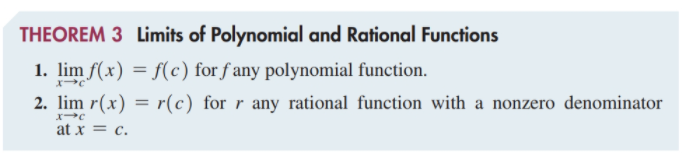
\includegraphics[width=0.9\linewidth]{9-1-5}
\end{center}

\subsubsection{Limit of a Quotient} If we have that the denominator of a qutient is zero while the numerator is non-zero, then the limit does not exists (is not finite).
\begin{center}
	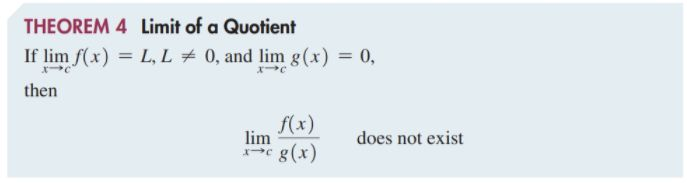
\includegraphics[width=0.9\linewidth]{9-1-6b}
\end{center}

\subsection{Indeterminate Form} Did you notice in our \textit{Properties of Limits} and in \textit{Rational Functions} that the denominator cannot be equal to zero? We will cover this case in the next section but if \textbf{both the denominator and the numerator are zero} we have an \textit{Indeterminate Form}. This does not state that the limit exists or does not exist but that we must investigate further.Typically, we use algebra to investigate further.
\begin{center}
	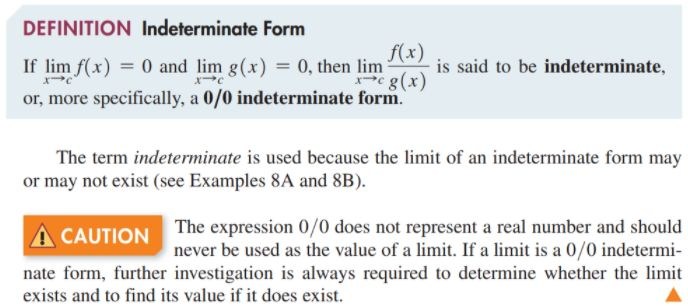
\includegraphics[width=0.9\linewidth]{9-1-6a}
\end{center}
\subsubsection{Examples}
\begin{align*}
	\lim_{x\to 2}\frac{x^2-4}{x-2} &= \frac{0}{0} \\
	\frac{x^2-4}{x-2} &= \frac{(x-2)(x+2)}{x-2} \tag{using algebra} \\
	&=(x+2) \\
	\lim_{x\to 2}(x+2) = 4
\end{align*}



\noindent\rule{\textwidth}{1pt}
{\footnotesize Copyright (C) 2021 Garold Dalton --- Released under GNU General Public License v3.0}


\cleardoublepage


\end{document}
